% =====================================================================
%  CITS4012 Group Project -- PIQA
%
%  Built from the official ACL LuaLaTeX template in preprint mode.
%
%  compact.sty holds every layout knob in one place -- float spacing,
%  caption size, display-maths skips. Turn those to trade whitespace
%  for pages without touching a word of the text.
% =====================================================================
\documentclass[11pt]{article}
\usepackage[preprint]{acl}
\usepackage{microtype}
\usepackage[english,bidi=default]{babel}
\babelfont{rm}{TeXGyreTermesX}
\usepackage{graphicx}
\usepackage{amsmath,amssymb}
\usepackage{booktabs}
\usepackage{colortbl}             % \rowcolor for the "Ours" rows in Table 3
\definecolor{ourrow}{RGB}{226,238,248}
\usepackage{url}
\usepackage{compact}              % all spacing knobs live here
\setcitestyle{authoryear,round}

\title{Attention over Near-Duplicate Candidates on PIQA:\\Separating Noise From Signal}
\author{Group 15}
\date{}

\begin{document}
\maketitle
\begin{abstract}
\noindent
The two candidate solutions of a PIQA instance are near-duplicates,
overlapping by $0.653$ on average, so we condition attention on the goal and
add a parameter-free residual aligning each candidate against the other.
Against a pooled seed-noise threshold of $0.0099$, no attention
configuration separates from a no-attention backbone. The baselines locate
the gain elsewhere: a frozen pretrained encoder scores below our model, the
same checkpoint fine-tuned $6.1$ points above it, and zero-shot Qwen2.5-3B
$18.0$ points above. At this data scale pretraining, not architecture, moves
the result.
\end{abstract}

\section{Introduction}
\label{sec:intro}

A PIQA instance gives a physical goal and two candidate solutions, exactly one
correct \citep{bisk2020piqa}. The candidates overlap by $0.653$ on average
across $16{,}113$ training instances, so the evidence lies in a few disputed
positions. Our shared BiLSTM keeps their scores on one scale; goal-conditioned
attention selects relevant candidate words; and a parameter-free residual
aligns each candidate against the other. Each component is ablated, with
differences judged against a $0.0099$ seed-noise threshold. The best attention
gain is only $0.0039$, and the flattest weights perform best; only pretraining
scale moves the result.

\section{Methodology}
\label{sec:method}

\subsection{Task formulation and notation}
\label{sec:task}

An instance is a goal $g$, candidates $s_1,s_2$ of which exactly one is
correct, and a label $y \in \{1,2\}$. We score rather than classify a
concatenated input: $f$ takes the goal, the candidate scored and the competing
candidate, returning an unnormalised real number:
\begin{equation}
\hat{y} \;=\; \operatorname*{arg\,max}_{k \in \{1,2\}} \; f(g,s_k,s_{3-k}).
\label{eq:argmax}
\end{equation}
A softmax over the two feeds the cross-entropy loss. Because both pass through
the same $f$, their scores share a scale and the prediction is independent of
their order.

\subsection{The characteristics of PIQA that drive the design}
\label{sec:hard}

\begin{figure}[tb]
  \centering
  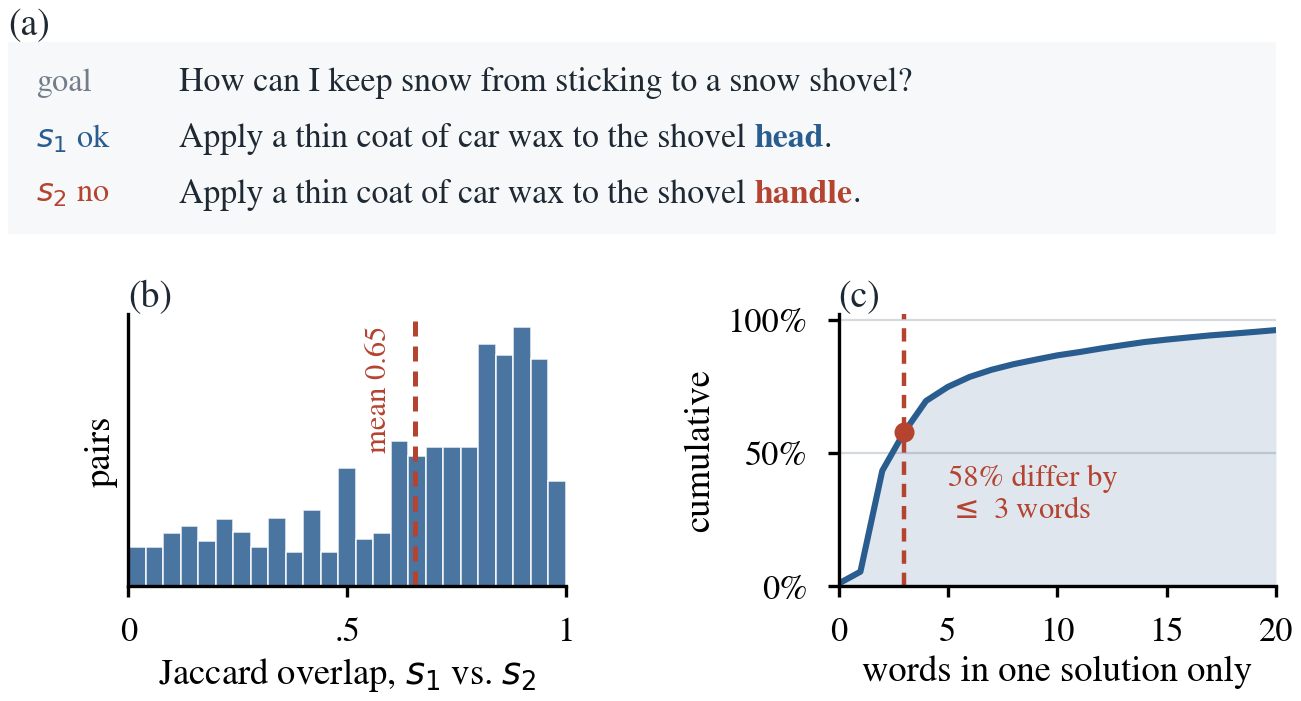
\includegraphics[width=0.82\columnwidth]{fig1_task.png}
  \caption{(a) A training instance whose candidates differ by one word.
  (b) Jaccard overlap of $s_1$ and $s_2$ over the $16{,}113$ training
  instances. (c) Cumulative distribution of words appearing in only one
  candidate.}
  \label{fig:task}
\end{figure}


Figure~\ref{fig:task} shows a one-word contrast and the corpus pattern behind
it. For distinct-token Jaccard overlap, $J = |W(s_1) \cap W(s_2)| /
|W(s_1) \cup W(s_2)|$, $37.5\%$ of pairs exceed $0.8$, and $57.9\%$ differ by
at most three words. Three decisions follow.

\begin{description}
  \item[D1] \textit{Share one encoder and scorer,} so candidate differences
  originate in the text rather than separate weights.
  \item[D2] \textit{The goal determines which words of a candidate matter.}
  It constructs the query because it is what makes one candidate correct.
  \item[D3] \textit{The candidates attend to each other.} The discriminative
  signal lies where they disagree, so the scorer receives that residual
  directly. This is our task-specific component.
\end{description}

\subsection{Shared encoder}
\label{sec:encoder}

Tokens pass through an embedding matrix $E$ of size $V$ by $d$, trained from
scratch. One bidirectional LSTM \citep{hochreiter1997lstm} encodes all three
inputs, giving states of size $L_g \times 2H$ and $L_s \times 2H$ with
$L_g = 20$, $L_s = 60$, $d = 100$, $H = 100$. Sharing the encoder implements
D1 and extends the Siamese arrangement of \citet{mueller2016siamese} from two
inputs to three; wherever a sequence is reduced to one vector we average over
non-padding positions.

A vanilla RNN was rejected for 60-token candidates; a GRU scores
$0.5922 \pm 0.0060$ versus the LSTM's $0.6003 \pm 0.0032$, inside the noise
floor. A Transformer was set aside on data scale: the original saw 4.5M
sentence pairs \citep{vaswani2017attention}, versus our $13{,}696$, with no
pretrained embeddings here.

\subsection{Attention over the candidate and over the goal}
\label{sec:attn}

All three share one form: a query $\mathbf{q}$ scores every position of a
sequence $H$, padding is suppressed before the softmax, and the weights pool
it:
\begin{equation}
\boldsymbol{\alpha} = \mathrm{softmax}\!\left(\frac{H\mathbf{q}}{T}\right),
\qquad
\mathbf{c} = \sum_i \alpha_i \mathbf{h}_i .
\label{eq:attn}
\end{equation}
The temperature $T$ controls concentration (Section~\ref{sec:refine}); $T = 1$
recovers the unscaled form. What distinguishes the mechanisms is where the
query comes from.

\paragraph{A1, goal-conditioned attention}
The goal gives $\mathbf{q}=Wg$, and $c_k$ summarises the candidate. This is
the general score of \citet{luong2015attention} applied across two sequences;
$W$ maps what is asked to what is proposed.

\paragraph{A2, self-attention over the goal}
Rather than average the goal, a learned 200-parameter query $q_g$ applies
Equation~\ref{eq:attn}, following \citet{yang2016hierarchical}.

\subsubsection{Refinements to goal-conditioned solution attention}
\label{sec:refine}

We refine A1 in three ways while leaving A2 unchanged, padding masks
suppressing invalid positions throughout. Each solution token first attends to
the non-padding goal tokens in a low-rank space ($r = 64$), adding a gated
residual with $\beta$ initialised to zero; the states are then pooled under a
learned temperature $T$ initialised to $\sqrt{D}$, and the attended context is
mixed with $\bar{h}_k$, the masked mean of the original states, through a gate
$\lambda = \sigma(\gamma)$ initialised to $0.5$:
\begin{align}
A_k &= \mathrm{softmax}_j\!\left(
   \tfrac{(H^{k}W_{Q})(H^{g}W_{K})^{\!\top}}{\sqrt{r}}
   + M^{g}\right), \nonumber\\
\widetilde{H}^{k} &= H^{k} + \tanh(\beta)\,A_k\!\left(H^{g}W_{V}\right)W_{O},
   \nonumber\\
\boldsymbol{\alpha}_k &= \mathrm{softmax}_i\!\left(
   \tfrac{\widetilde{H}^{k}\mathbf{q} + M^{k}}{T}\right), \nonumber\\
c_k &= \lambda\,\boldsymbol{\alpha}_k^{\!\top}\widetilde{H}^{k}
       + (1-\lambda)\,\bar{h}_k .
\label{eq:refine}
\end{align}
The zero-initialised residual initially has no effect and only changes A1.
This adaptation of scaled dot-product attention \citep{vaswani2017attention}
adds $51{,}203$ parameters: four projections at $D=200$ and three scalars.

\subsection{Cross-attention between the candidates}
\label{sec:cross}

A3 implements D3 by aligning each token of one candidate with every
non-padding token of the other \citep{chen2017esim}, keeping the signed
residual $r^{k}_{i} = h^{k}_{i} - \sum_j \beta^{k}_{ij} h^{3-k}_{j}$ between a
token and what the competing candidate explains of it:
\begin{equation}
d_k = \left[\begin{array}{c}
  \mathrm{maskedMean}_i(r^{k}_{i})\\[-1pt]
  \mathrm{maskedMax}_i(r^{k}_{i})
\end{array}\right] \in \mathbb{R}^{4H},
\label{eq:residual}
\end{equation}
with $\beta^{k}_{ij}=\mathrm{softmax}_j((h^{k}_{i})^{\!\top}h^{3-k}_{j})$
unscaled over the original states, independent of A1. Mean and max preserve
distributed and local differences without new parameters. Unlike ESIM, the
candidates are symmetric, so we pool the residual directly without a second
recurrent layer.

\subsection{Interaction features and scoring}
\label{sec:scoring}

The goal, attended candidate summary and alignment residual combine through
the interaction features of \citet{conneau2017infersent}:
\begin{equation}
u_k = \big[\, g; \; c_k; \; g \odot c_k; \; |g - c_k|; \; d_k \,\big]
      \in \mathbb{R}^{12H}.
\label{eq:u}
\end{equation}
Product and absolute difference expose agreement and disagreement; a two-layer
network maps $u_k$ to a scalar. The complete model (Figure~\ref{fig:arch}) has
$1{,}522{,}204$ parameters, $75.5\%$ in its embedding matrix.

\begin{figure*}[tb]
  \centering
  \includegraphics[width=0.76\textwidth]{fig2_architecture.pdf}
  \caption{Model architecture. One embedding matrix and one bidirectional LSTM
  encode all three inputs; one scorer is applied to each candidate in turn.
  A3 adds no parameters, though the max-pooled half of $d_k$ widens the
  scorer input to $12H$.}
  \label{fig:arch}
\end{figure*}

\section{Experimental Setup}
\label{sec:setup}

\subsection{Dataset and preprocessing}
\label{sec:data}

PIQA provides $16{,}113$ labelled training and $1{,}838$ test instances with
no official validation split; neither favours one answer position
(Table~\ref{tab:data}), so accuracy is not inflated by a class prior.

\begin{table}[tb]
  \centering\footnotesize
  \begin{tabular}{@{}lrr@{}}
    \toprule
     & \textbf{train} & \textbf{test}\\
    \midrule
    Instances & $16{,}113$ & $1{,}838$\\
    Proportion with $y = 2$ & $0.500$ & $0.505$\\
    Goal words, mean / p95 & $7.1$ / $13$ & n/m\\
    Candidate words, mean / p95 & $19.6$ / $54$ & n/m\\
    Jaccard overlap, mean & $0.653$ & n/m\\
    Candidates differing by $\leq 3$ words & $57.9\%$ & n/m\\
    Vocabulary, count $\geq 2$ & $11{,}488$ & ---\\
    \bottomrule
  \end{tabular}
  \caption{Dataset statistics; candidate length is the longer of the two.
  Entries marked n/m were deliberately not measured (see text).}
  \label{tab:data}
\end{table}

\paragraph{Splits}
An $85/15$ label-stratified split gives $13{,}696$ training and $2{,}417$
validation instances. All design and ablation choices use that split; the test
set was used once for Table~\ref{tab:overall}, after inspecting only its size
and label balance.

\paragraph{Preprocessing}
After lower-casing and punctuation removal, text is split on whitespace. The
training-only vocabulary has $11{,}488$ types at count $\geq2$ plus unknown;
$L_g=20$ and $L_s=60$ exceed the 95th percentiles, truncating $0.2\%$ of goals
and $3.5\%$ of candidates.

\subsection{Training procedure}
\label{sec:training}

Models train with Adam \citep{kingma2015adam}, batch size $32$, cross-entropy,
and scorer-input dropout. Per-parameter steps suit a dominant embedding matrix
whose rows update only when their words occur.

\paragraph{Epoch budget}
Every configuration trains for a fixed $15$ epochs and we keep the epoch of
highest validation accuracy. Over ten seeds run to $25$, the mean curve
flattens by the fifth, individual runs peak at a median of $13.5$ epochs, and
extending the budget is worth $0.0019$, inside the noise floor below
(Figure~\ref{fig:epoch-budget}).

\begin{figure}[tb]
  \centering
  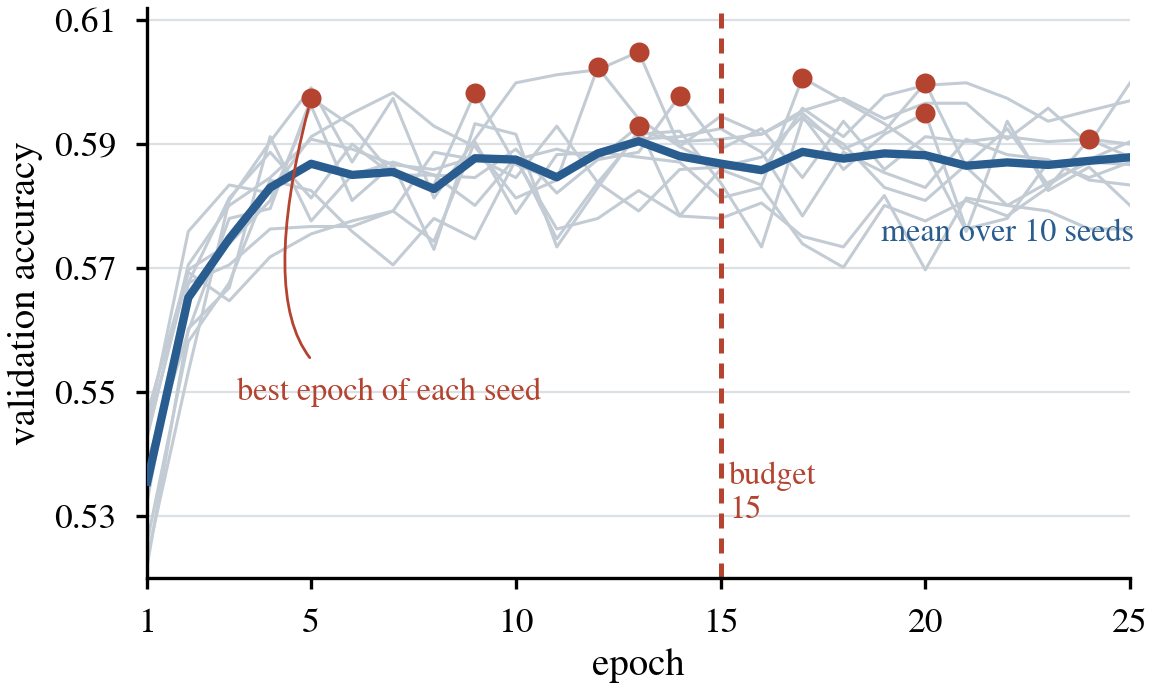
\includegraphics[width=\columnwidth]{fig3_convergence.png}
  \caption{Validation accuracy of the reference configuration over $25$
  epochs for ten seeds. Grey lines show individual runs, the blue line their
  mean, red markers each run's best epoch, and the dashed line the $15$-epoch
  budget used throughout.}
  \label{fig:epoch-budget}
\end{figure}

\paragraph{Reproducibility}
We seed Python, NumPy and PyTorch, set \texttt{cudnn.deterministic}, and disable
\texttt{cudnn.benchmark}. These controls reduced same-seed drift of up to
$0.015$ to exact reproduction. Runs used one Tesla T4, torch 2.11.0+cu130.

\paragraph{Noise floor}
Across sixteen configurations, three-seed standard deviations span $0.0002$
to $0.0083$. Pooling them gives $0.0049$; mean gaps below twice that,
$0.0099$, are not separable, and larger gaps receive Welch's $t$-test.

\subsection{Hyperparameter selection}
\label{sec:hparams}

Hyperparameters were selected one at a time around a fixed reference
configuration, on the validation split with attention disabled
(Figure~\ref{fig:hp}).

\begin{figure*}[tb]
  \centering
  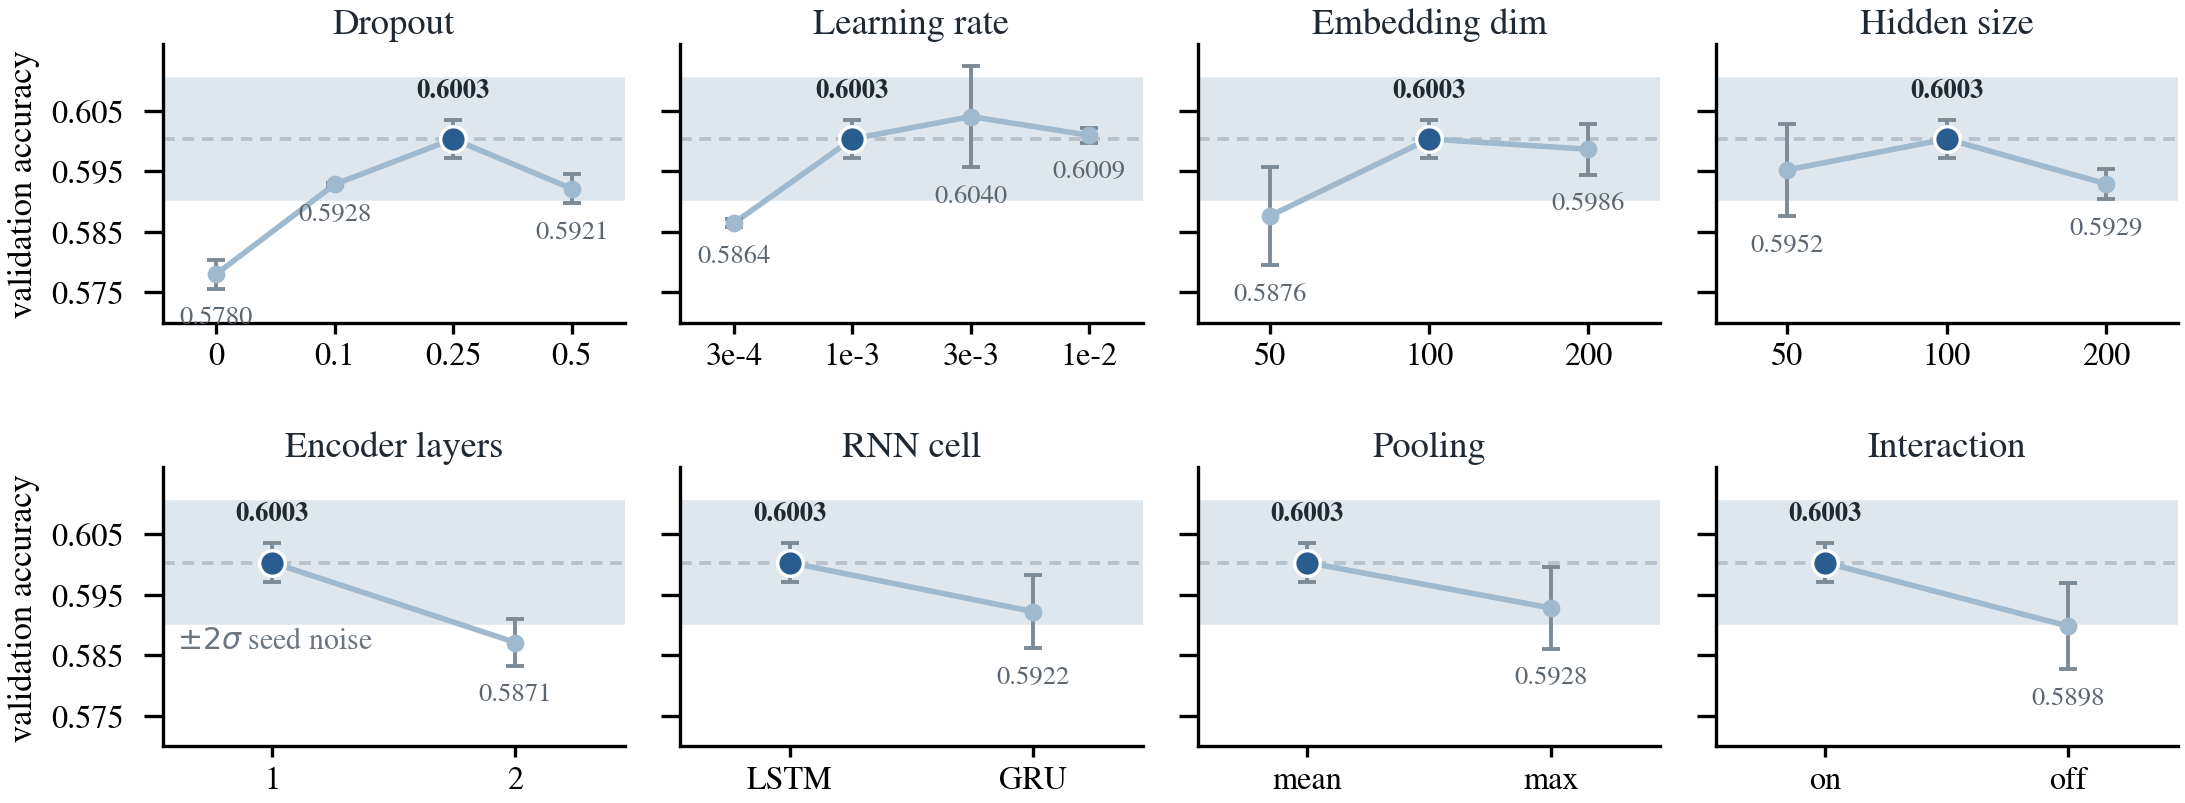
\includegraphics[width=0.78\textwidth]{fig4_hyperparams.png}
  \caption{Validation accuracy for every hyperparameter value tested around
  the no-attention reference. Three seeds per point; error bars one standard
  deviation, dashed line the reference, shaded band two pooled standard
  deviations of seed noise, dark marker the value adopted.}
  \label{fig:hp}
\end{figure*}


The adopted configuration is dropout $0.25$, learning rate $0.001$, embedding
width $100$, hidden size $100$, one encoder layer, an LSTM cell, mean pooling,
interaction features on, batch size $32$ and $15$ epochs. Only three settings
fall outside the noise band: removing dropout costs $0.0223$, a second encoder
layer $0.0133$, and removing the interaction features $0.0105$. The other
eight sit inside it, and there we took the simpler setting --- learning rate
$0.003$
scored $0.0037$ above $0.001$ but with a seed spread two and a half times
wider, and hidden size was flat, so we took the smallest value on that
plateau.

\subsection{Baseline models}
\label{sec:baselines}

Four self-run baseline families span adaptation: B1 bag-of-embeddings, B2a/B2b
the same DistilRoBERTa frozen/fine-tuned, and B3 zero-shot Qwen2.5-3B
\citep{qwen2024}. They use the same split and seeds; Figure~\ref{fig:base}
plots both splits.

\begin{figure}[tb]
  \centering
  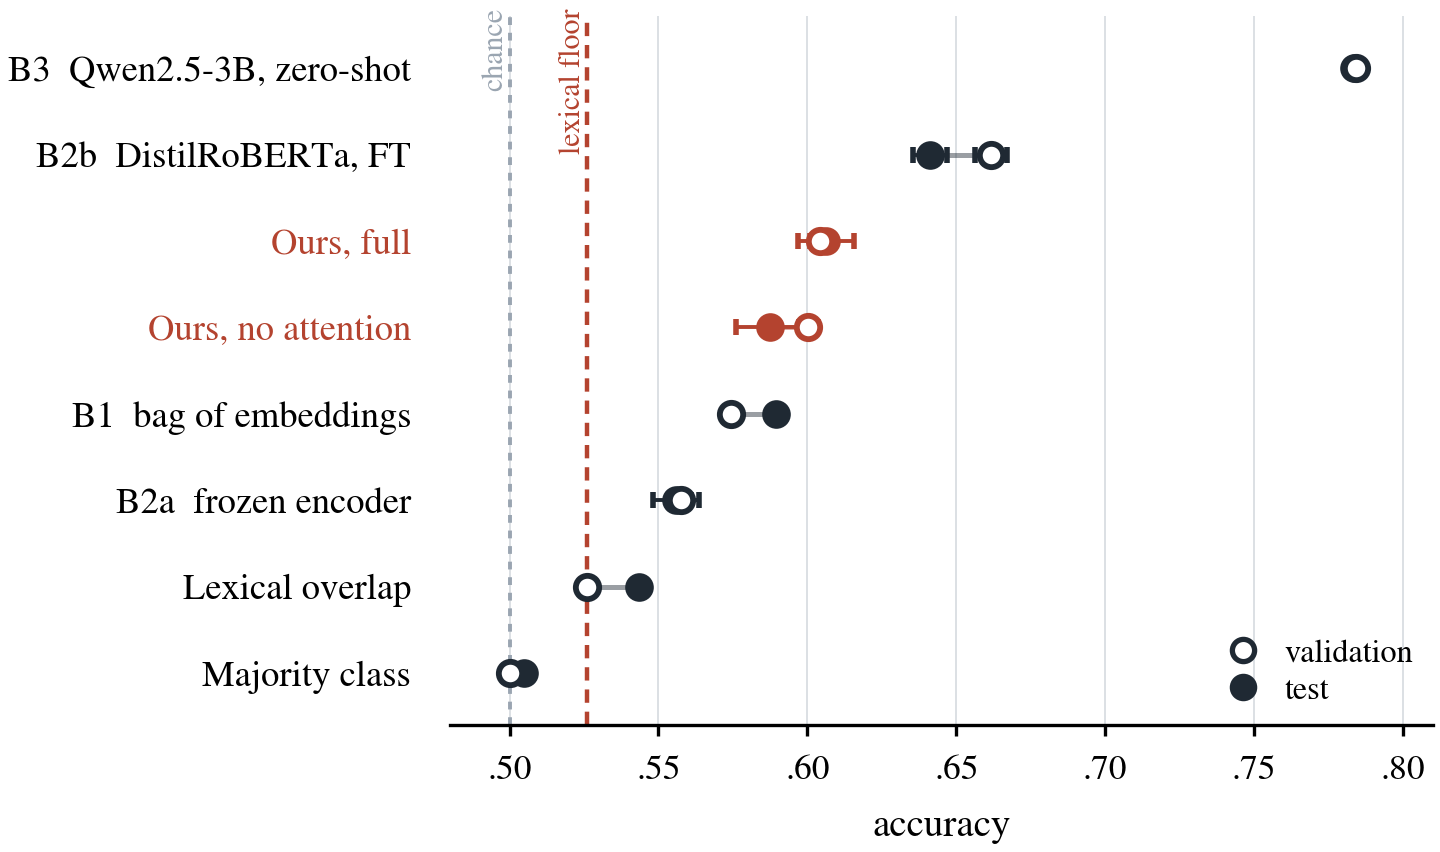
\includegraphics[width=0.80\columnwidth]{fig5_baselines.png}
  \caption{Validation (hollow) and test (filled) accuracy per system, error
  bars one standard deviation over three seeds. Dashed lines mark the majority
  baseline and the lexical floor; the axis is truncated at $0.48$.}
  \label{fig:base}
\end{figure}

\paragraph{B0, the lexical floor}
A heuristic selecting whichever candidate shares more words with the goal
reaches $0.5259$ on validation, the floor a learned model must clear.

\paragraph{B1, bag of embeddings}
B1 replaces the BiLSTM by a masked mean over embeddings, retaining the
Section~\ref{sec:scoring} features except $d_k$.

\paragraph{B2a, frozen pretrained encoder}
All 82M parameters of \texttt{distilroberta-base}
\citep{sanh2019distilbert,liu2019roberta} are frozen; only a 769-parameter
classifier over each $(g,s_k)$ \texttt{[CLS]} vector trains for five epochs
at $10^{-3}$, batch size 16 and 10\% warmup.

\paragraph{B2b, fine-tuned pretrained encoder}
B2b changes one variable: it unfreezes the encoder. Pairs truncate to 128
subwords in \texttt{AutoModelForMultipleChoice}; AdamW uses $2\times10^{-5}$
and linear decay after warmup \citep{mosbach2021stability}.

\paragraph{B3, Qwen2.5-3B zero-shot}
In one deterministic fp16 run, B3 scores each candidate by mean token
log-likelihood under \texttt{Qwen/Qwen2.5-3B-Instruct} and the fixed prompt
\texttt{Goal: \{g\}\textbackslash nSolution: \{s\_k\}}, following
\citet{bisk2020piqa}. Its web-scale corpus may contain PIQA-like text, so this
is pretraining headroom, not an architectural control.

\subsection{Evaluation metrics}
\label{sec:metrics}

Accuracy is the proportion whose score argmax matches gold. Labels are
balanced and the two errors --- choosing $s_1$ for $s_2$, or the reverse ---
have equal cost, so neither candidate is a privileged positive class.
Accuracy is therefore natural and matches PIQA \citep{bisk2020piqa};
macro-$F_1$ is monotone here.

\section{Results and Analysis}
\label{sec:results}

\subsection{Ablation studies}
\label{sec:ablation}

Table~\ref{tab:ablation} tests three hypotheses: alone, A1 should select
solution evidence, A2 goal evidence and A3 candidate differences; staged A1
tests mean preservation, softmax scaling, learned temperature and token-level
goal conditioning; leave-one-out rows test A2/A3 conditionally. Split,
backbone, scorer, optimiser, 15-epoch budget and seeds $0,1,2$ stay fixed,
with no attention as reference.

\begin{table}[tb]
  \centering\footnotesize
  \begin{tabular}{@{}lcc@{}}
    \toprule
    \textbf{Configuration} & \textbf{Validation} & \textbf{$\Delta$}\\
    \midrule
    No attention (reference) & $0.6003 \pm 0.0032$ & $0.0000$\\
    A1 (learned-query)       & $0.5901 \pm 0.0034$ & $-0.0102$\\
    A2 only                  & $0.5919 \pm 0.0029$ & $-0.0084$\\
    A3 only                  & $0.5999 \pm 0.0053$ & $-0.0004$\\
    A2 + A3                  & $0.6042 \pm 0.0069$ & $+0.0039$\\
    \midrule
    A1 + mean mix            & $0.5870 \pm 0.0046$ & $-0.0133$\\
    \;\;+ fixed $\sqrt{D}$ scaling & $0.5938 \pm 0.0011$ & $-0.0065$\\
    \;\;+ learned temperature      & $0.5959 \pm 0.0025$ & $-0.0044$\\
    Final A1                 & $0.5963 \pm 0.0034$ & $-0.0040$\\
    \midrule
    Full $-$ A2              & $0.5999 \pm 0.0030$ & $-0.0004$\\
    Full $-$ A3              & $0.5918 \pm 0.0054$ & $-0.0085$\\
    Full model               & $0.6042 \pm 0.0032$ & $+0.0039$\\
    \bottomrule
  \end{tabular}
  \caption{Validation ablations against the no-attention reference, mean $\pm$
  population standard deviation over seeds $0,1,2$. Final A1 $=$ mean mix $+$
  learned $T$ $+$ full-goal residual; Full $=$ that plus A2 and A3.}
  \label{tab:ablation}
\end{table}

Only learned-query A1 and unscaled A1 with mean mixing cross the $0.0099$
threshold, both negatively. The full model and A2$+$A3 share the highest mean
but gain only $0.0039$: no separable attention effect.

Scaling recovers $0.0069$ fixed and $0.0090$ learned in paired comparisons but
never beats no attention. The first A1 row uses a learned query, so its gap to
later goal-conditioned variants is not mixing alone. The refinements follow
scaled attention \citep{vaswani2017attention}, learned temperature
\citep{dufter2020temperature}, query-aware token representations
\citep{seo2017bidaf}, and a zero-initialised ReZero gate
\citep{bachlechner2021rezero}.

Removing A2 from the full model costs $0.0043$; removing A3 costs $0.0124$
($t=-2.79$), suggesting a conditional effect (Figure~\ref{fig:abl}). Yet with
three seeds, Full~$-$~A3 is within $0.0099$ of the reference and A3 alone is
$-0.0004$. We retain the full model for its joint-best mean, not a proven
attention advantage.

\begin{figure}[tb]
  \centering
  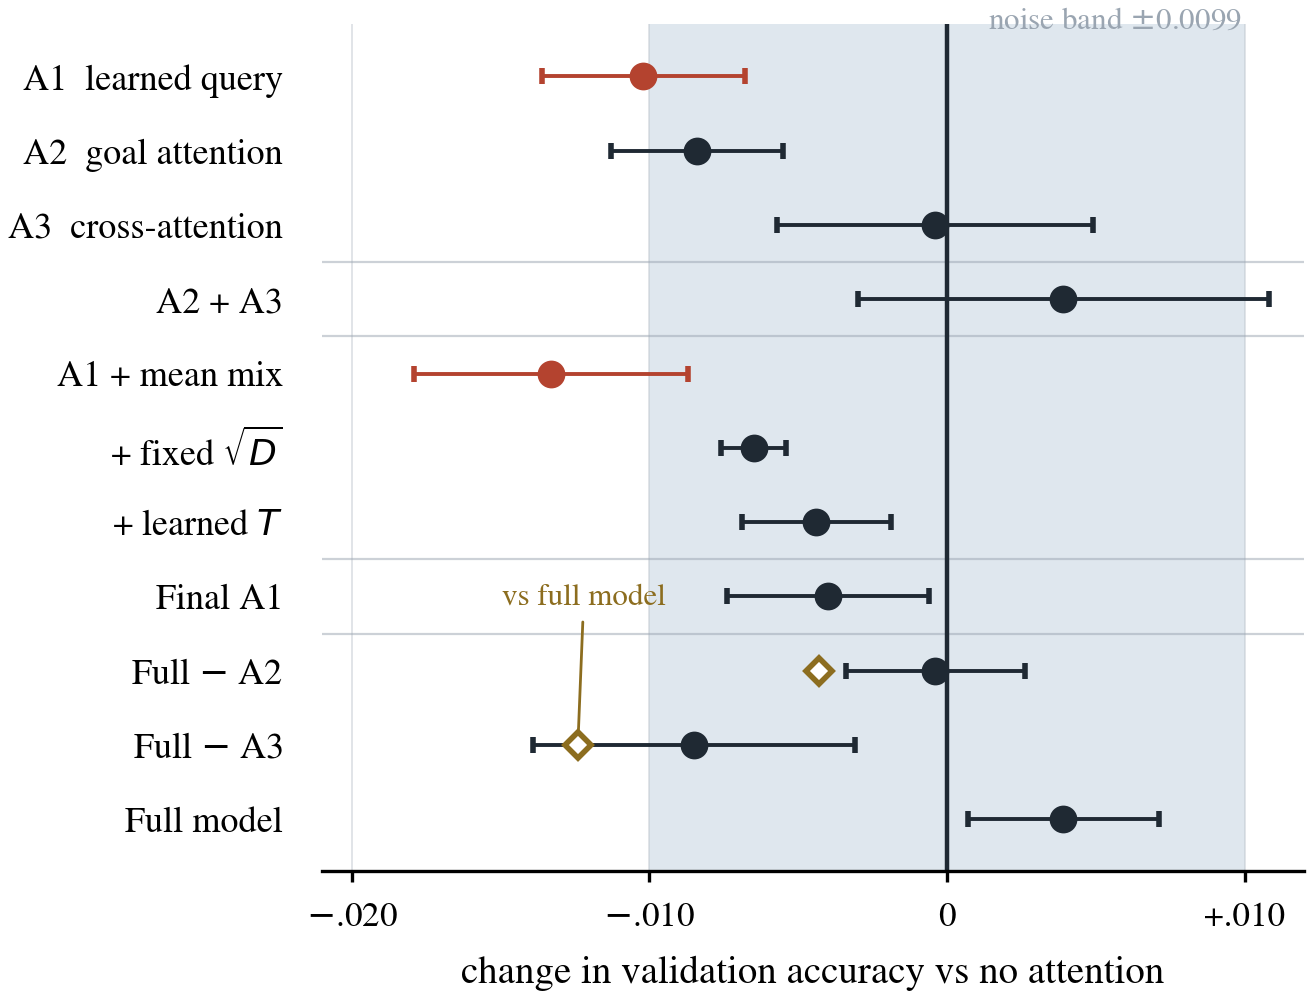
\includegraphics[width=0.80\columnwidth]{fig6_ablation.png}
  \caption{Attention ablations against the no-attention reference, error bars
  one standard deviation over three seeds. The shaded band spans the $0.0099$
  threshold; the two red points are the only configurations outside it, both
  negative. Open diamonds give the leave-one-out difference from the full
  model.}
  \label{fig:abl}
\end{figure}

\subsection{Qualitative analysis of attention}
\label{sec:qual}

On row $0$ --- remove potato sprouts; gold and all predictions: vegetable
peeler --- scaled A1 peaks at $0.056$--$0.063$ versus uniform $0.043$
(Figure~\ref{fig:temp}). Unscaled A1 reaches $0.126$ but favours shared words
such as \textit{peeling}; scaling makes it resemble mean pooling.


\begin{figure}[tb]
  \centering
  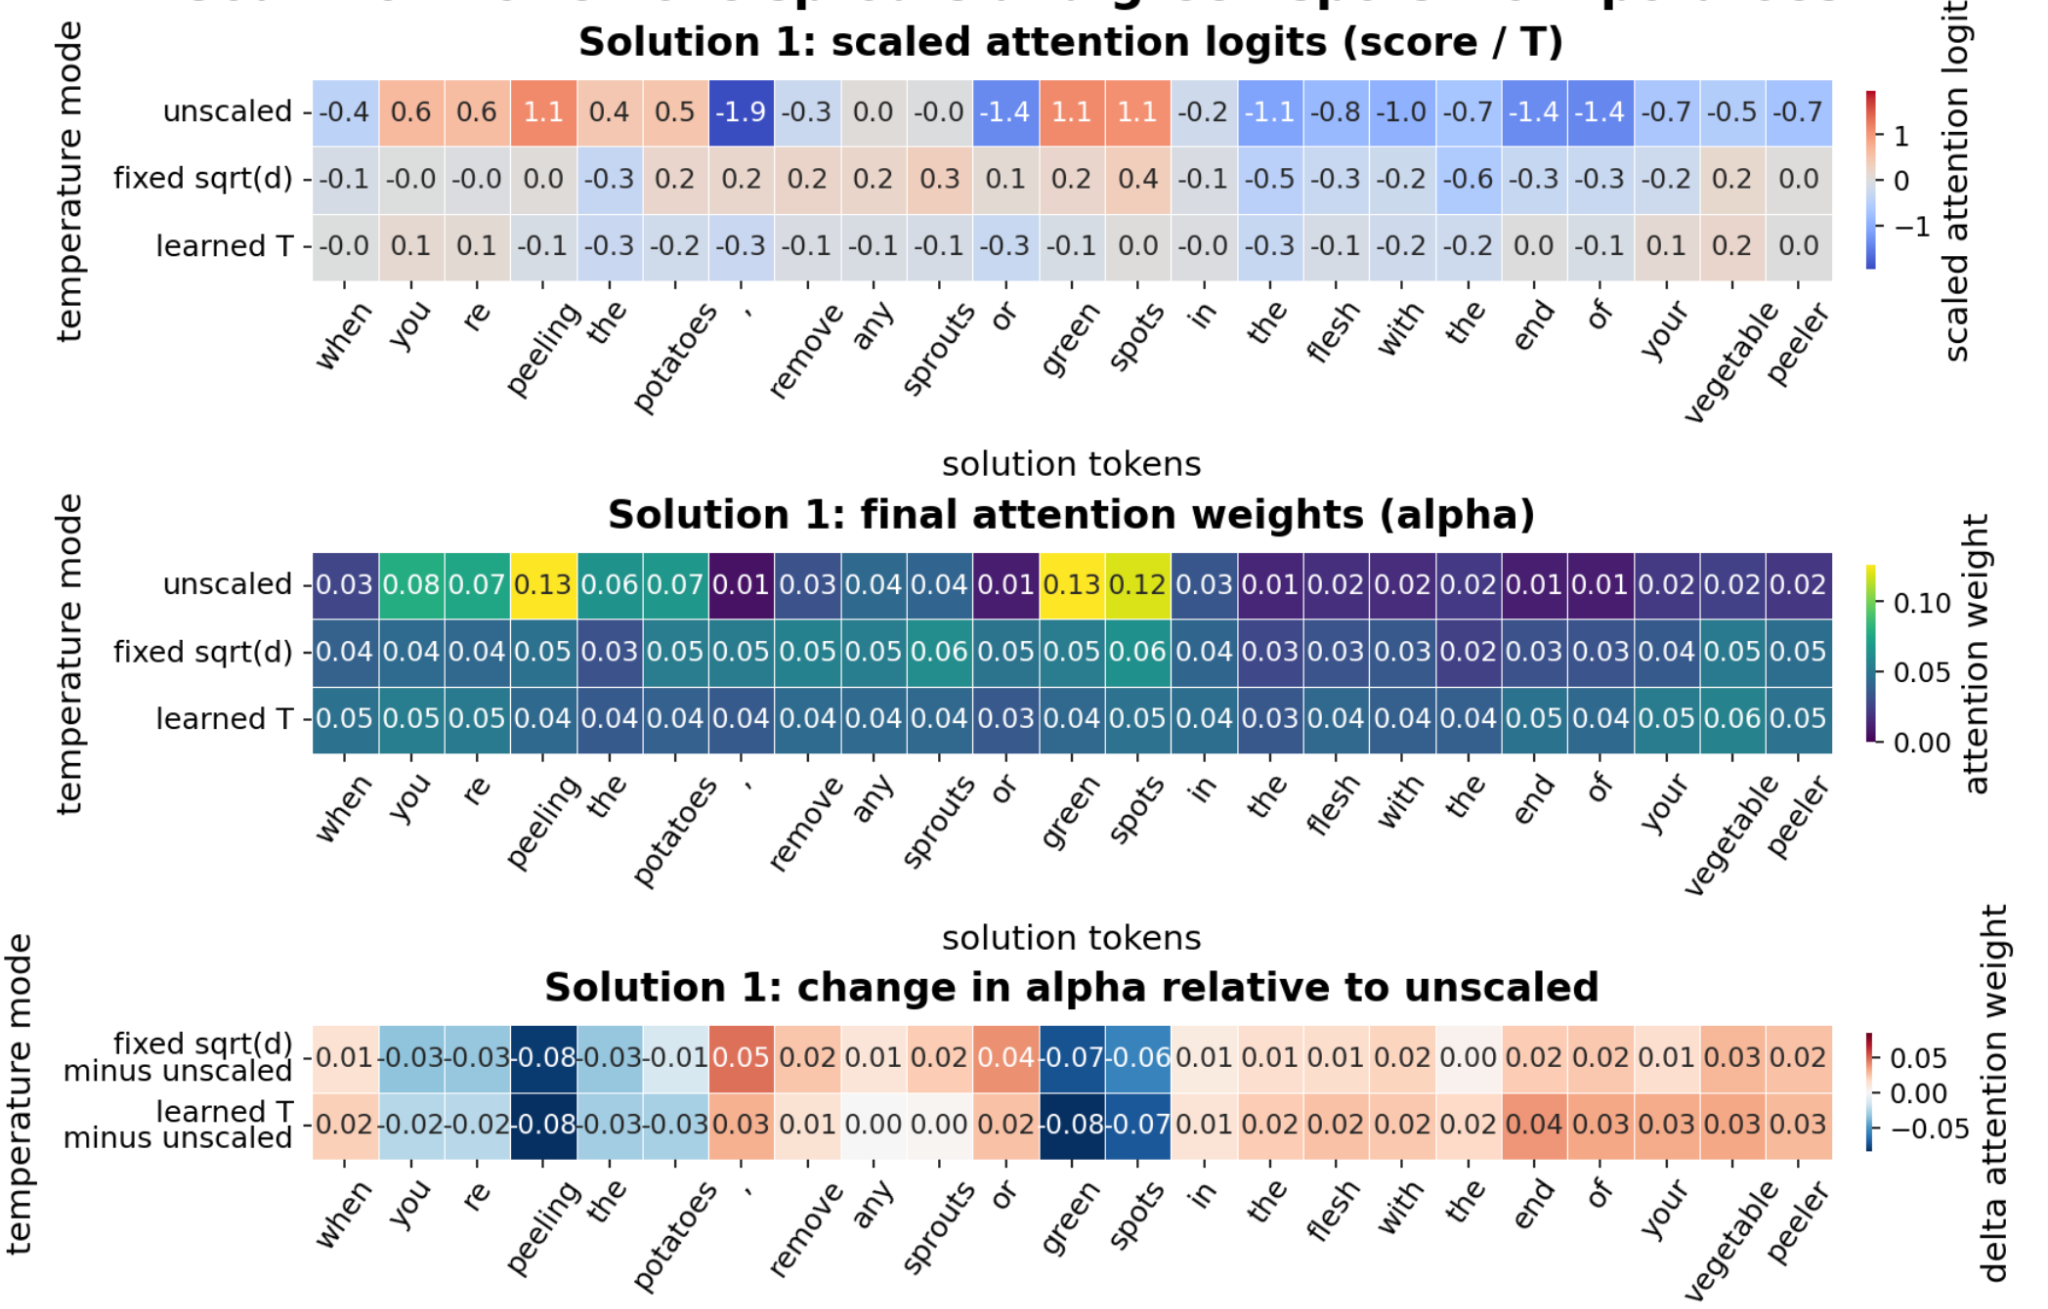
\includegraphics[width=\columnwidth]{fig7a_temp_sol1.png}
  \caption{A1 under three temperature settings, validation row $0$,
  solution~1: scaled logits, final weights $\alpha$, and the change in
  $\alpha$ against the unscaled checkpoint. Solution~2 behaves alike.}
  \label{fig:temp}
\end{figure}

On row $635$, goal \textit{Loosen stuck drawers}, solution~1 applies soap to
handles and solution~2 to runners. Gold is solution~2: the full model selects
it ($P=0.617$), while A1$+$mean mix predicts solution~1 ($P=0.938$).

\begin{figure}[tb]
  \centering
  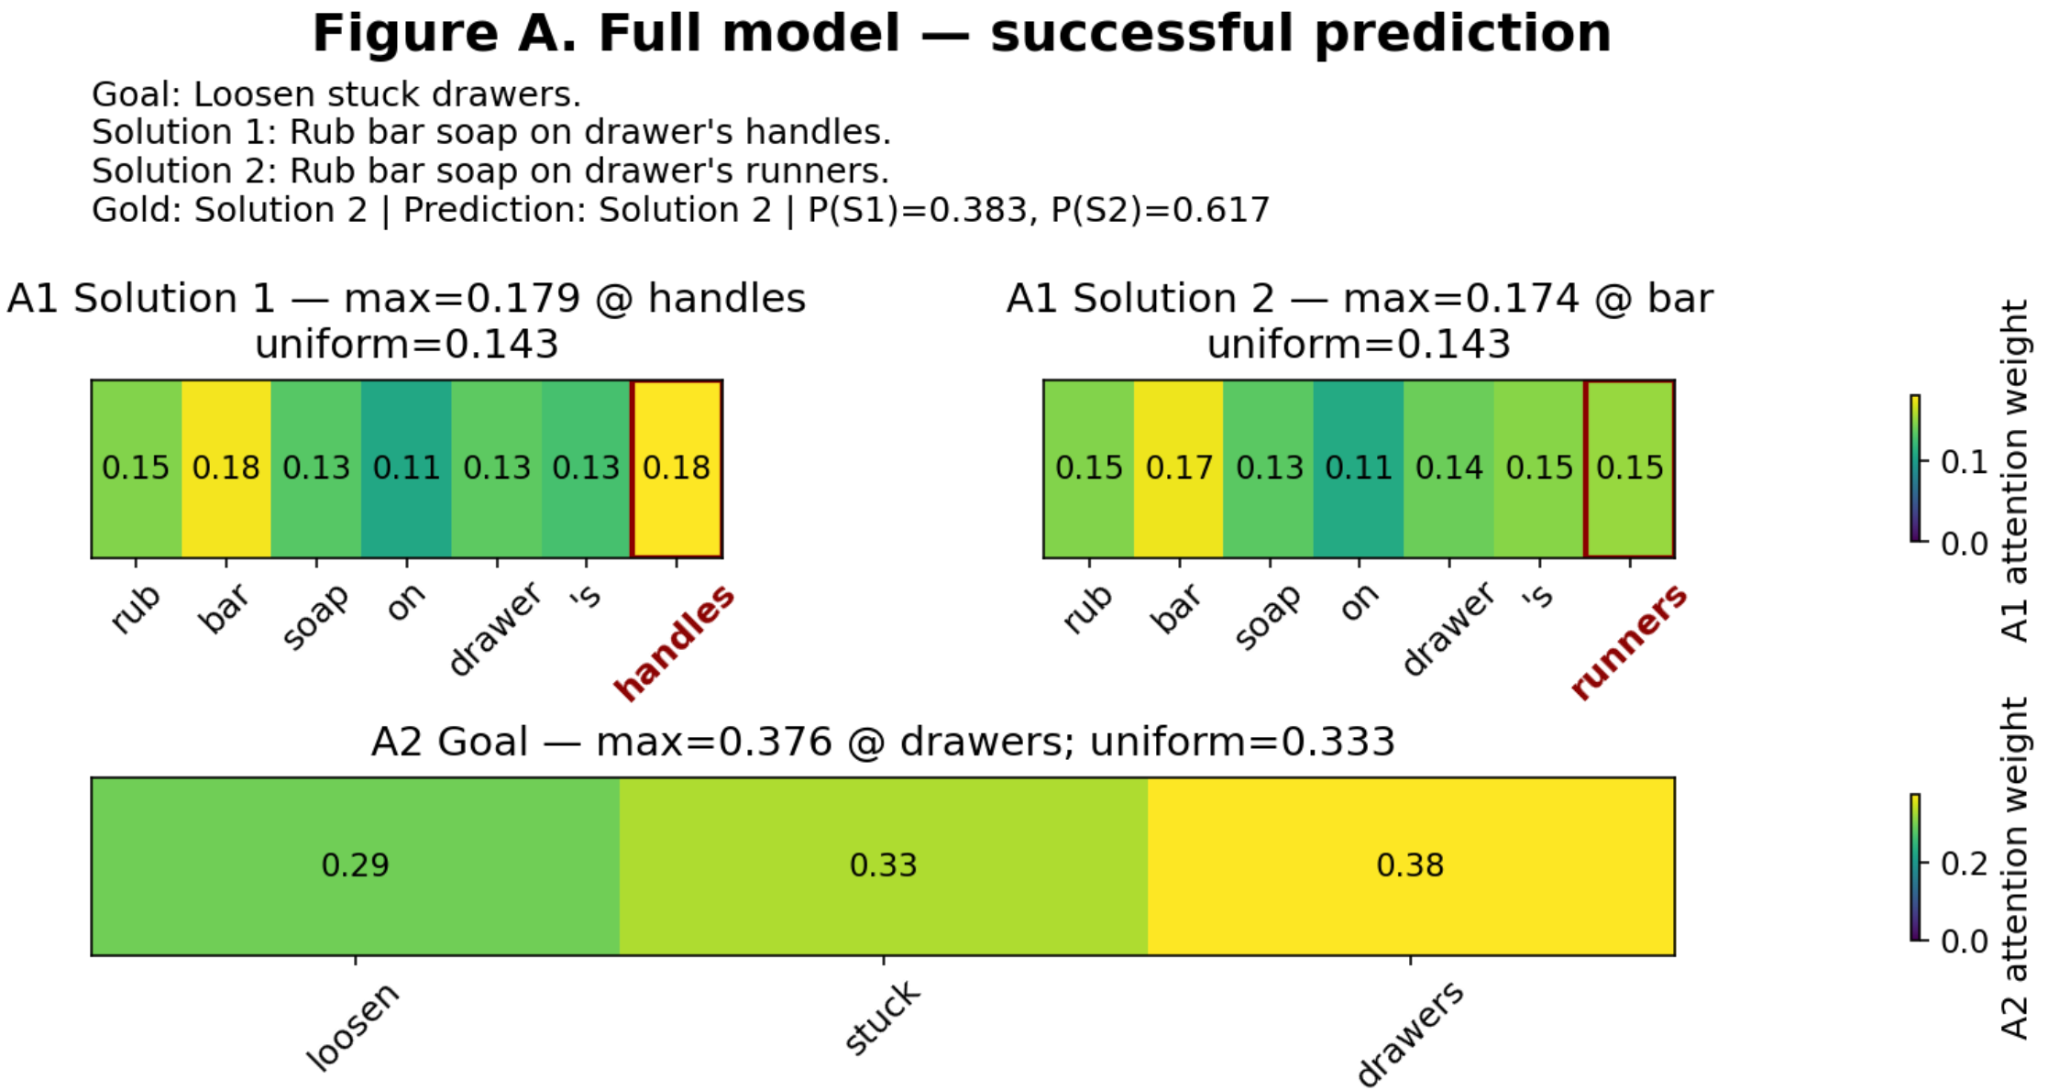
\includegraphics[width=0.93\columnwidth]{fig8a_full_a1a2.png}\\[1pt]
  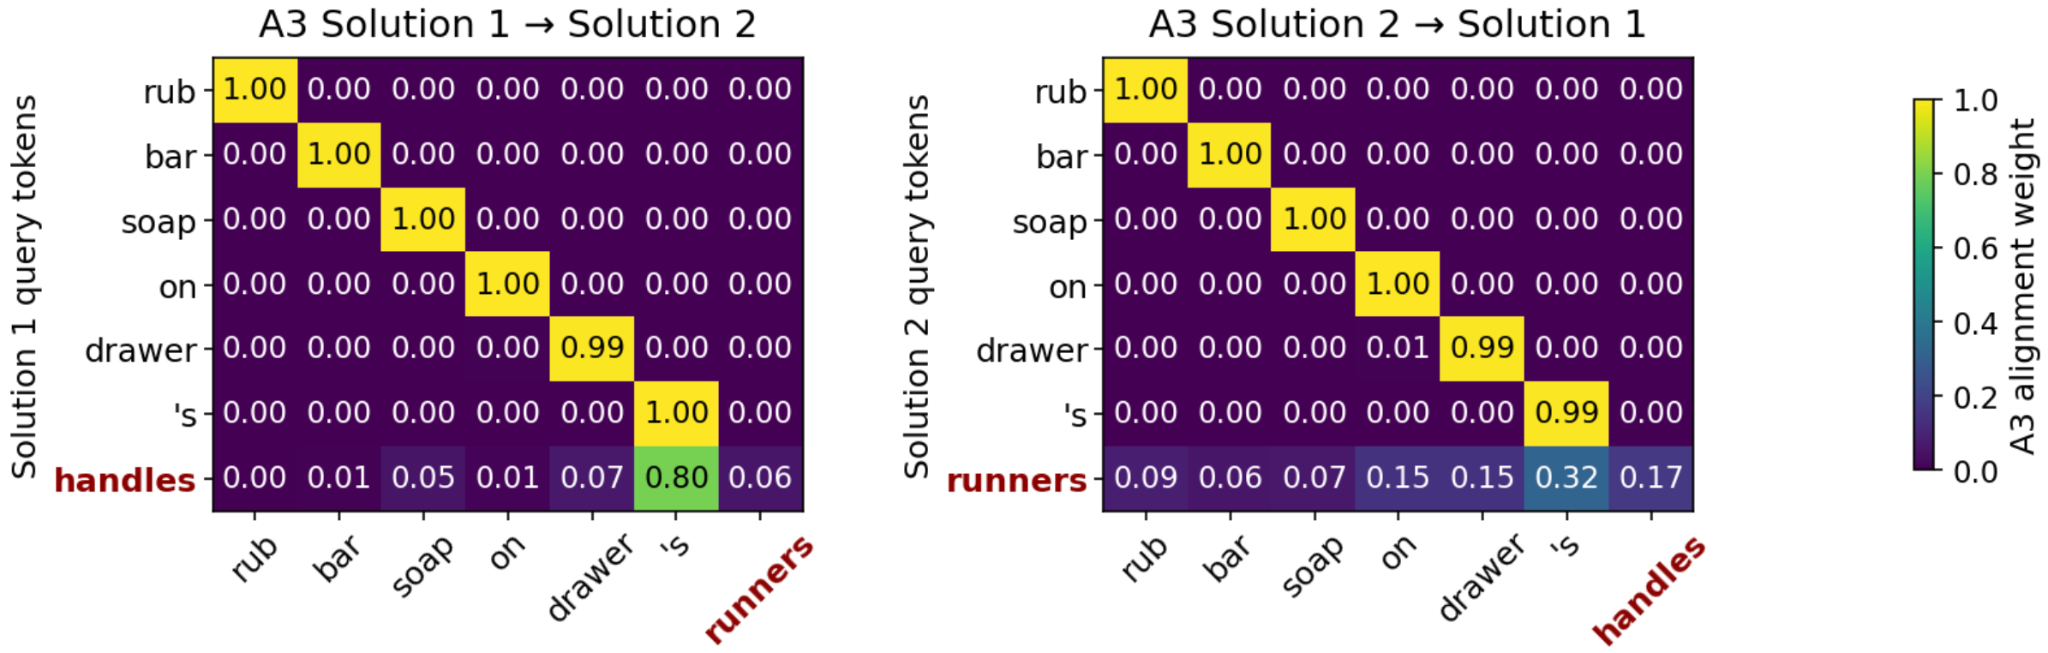
\includegraphics[width=0.93\columnwidth]{fig8b_full_a3.png}
  \caption{Full model on the correct prediction, validation row $635$. Top:
  A1 solution and A2 goal attention. Bottom: A3 cross-solution alignment, red
  labels marking tokens outside shared SequenceMatcher blocks (not learned
  signals).}
  \label{fig:heat1}
\end{figure}

In the success, A1 peaks at $0.179/0.174$ versus uniform $0.143$ and A2 is
also diffuse. A3 has structure: six shared tokens align at $0.99$--$1.00$,
exposing \textit{handles}/\textit{runners} without deciding which wins.

\begin{figure}[tb]
  \centering
  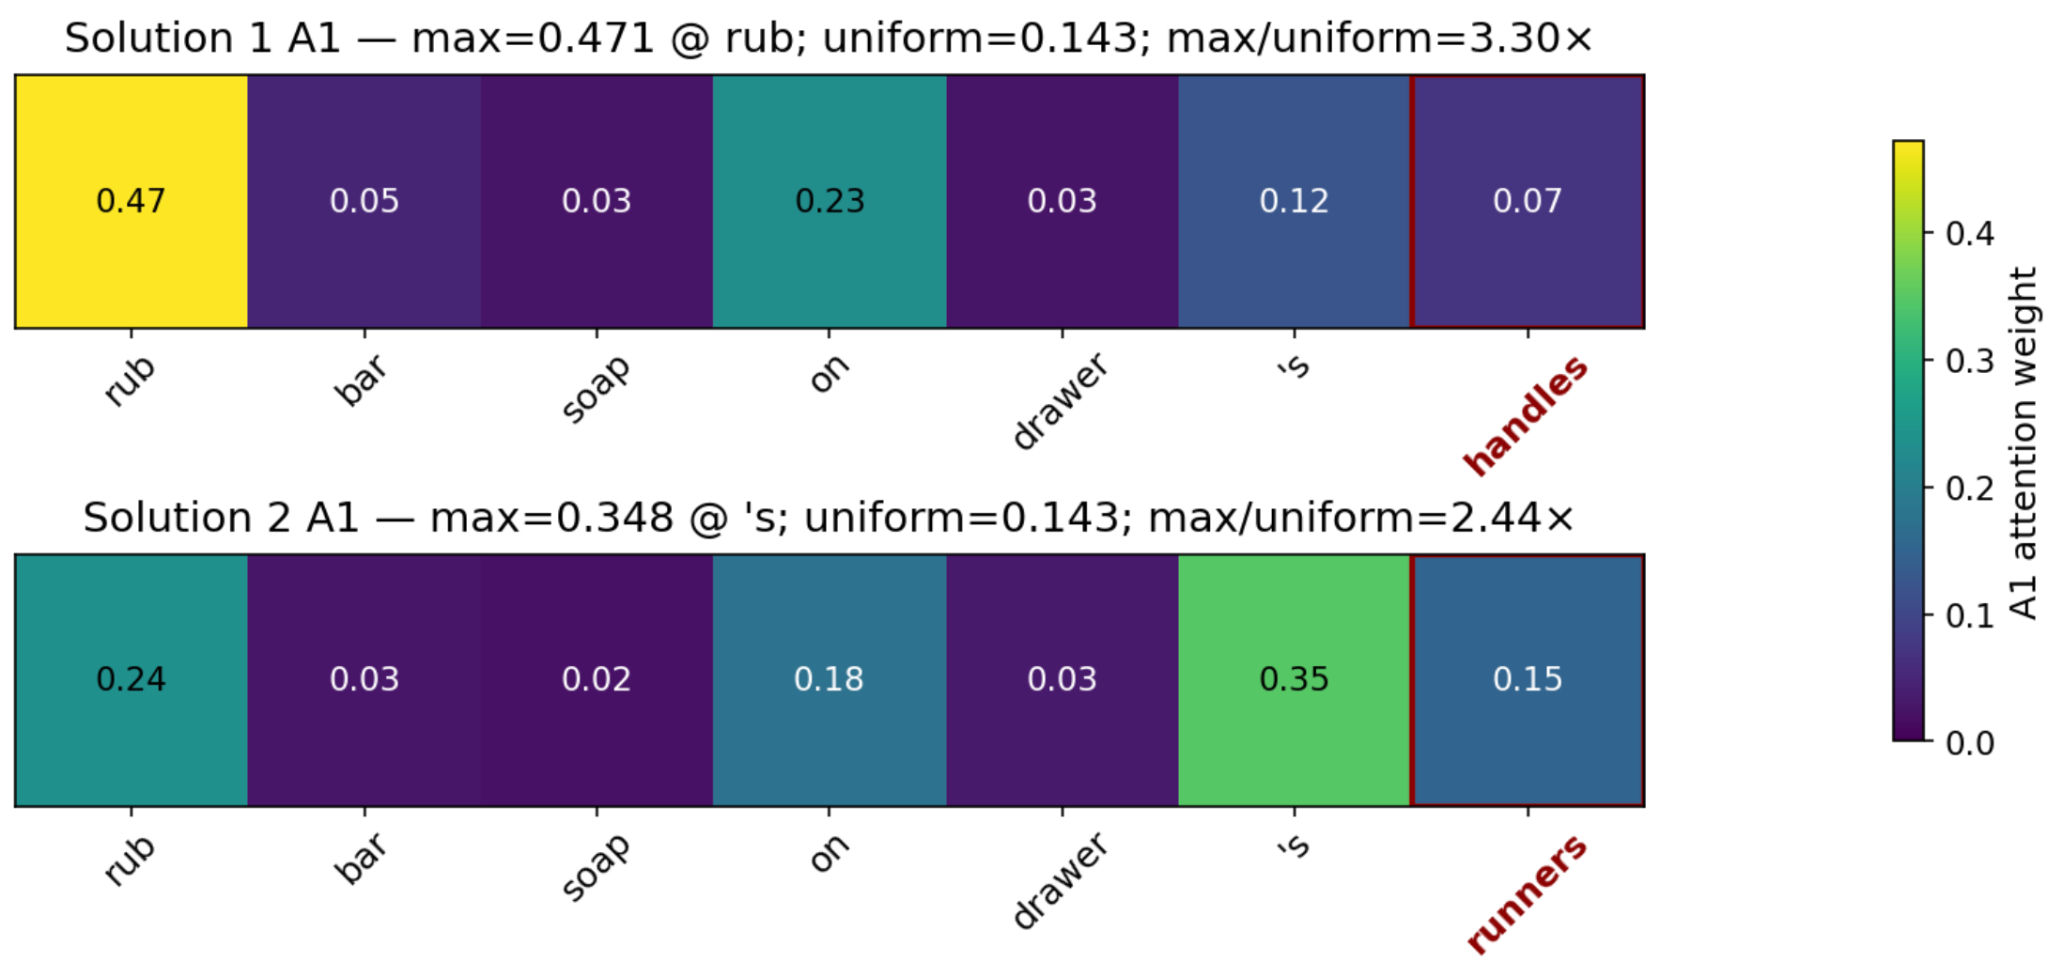
\includegraphics[width=0.93\columnwidth]{fig8c_ablation_err.png}
  \caption{A1 attention for the A1 $+$ mean mix ablation's highest-confidence
  error, validation row $635$. This configuration has neither A2 nor A3.}
  \label{fig:heat3}
\end{figure}

The failed ablation puts $0.471$ on shared \textit{rub} ($3.30\times$ uniform)
but only $0.071/0.151$ on the contrasting nouns; mixing weight $0.810$ lets
this dominate the mean. Thus sharpness is not a proxy for reasoning. These
different checkpoints describe behaviour, not a causal component effect.

\subsection{Overall performance comparison}
\label{sec:overall}

\begin{table}[tb]
  \centering\footnotesize
  \setlength{\tabcolsep}{0.8pt}
  \begin{tabular}{@{}lcc@{}}
    \toprule
    \textbf{System} & \textbf{Validation} & \textbf{Test}\\
    \midrule
    Majority class & $0.5002$ & $0.5049$\\
    Lexical overlap & $0.5259$ & $0.5435$\\
    \midrule
    B1 \ bag of embeddings & $0.5745 \pm 0.0023$ & $0.5896 \pm 0.0019$\\
    B2a \ frozen encoder & $0.5576 \pm 0.0034$ & $0.5559 \pm 0.0077$\\
    \midrule
    \rowcolor{ourrow}
    \textbf{Ours, no attention} & $0.6003 \pm 0.0032$ & $0.5874 \pm 0.0094$\\
    \rowcolor{ourrow}
    \textbf{Ours, full} & $0.6042 \pm 0.0032$ & $\mathbf{0.6063 \pm 0.0094}$\\
    \midrule
    B2b \ DistilRoBERTa, FT & $0.6617 \pm 0.0054$ & $0.6411 \pm 0.0057$\\
    B3 \ Qwen2.5-3B, 0-shot & $0.7844$ & $0.7835$\\
    \bottomrule
  \end{tabular}
  \caption{Accuracy on both splits, grouped by family rather than ranked.
  Learned systems use seeds $0,1,2$ with population standard deviations, both
  columns from one execution; the first two rows and B3 are deterministic.
  Separability threshold $0.0099$ on validation, $0.0187$ on test.}
  \label{tab:overall}
\end{table}

Four results follow from Table~\ref{tab:overall}. \textbf{(1)} Every validation
step clears the noise threshold except attention: its $0.0039$ gain has
$|t|=1.21$. \textbf{(2)} The frozen checkpoint is $4.27$ points below our
from-scratch model, but fine-tuning moves it $6.14$ above; that controlled
$10.41$-point step exceeds every architectural effect, while zero-shot
Qwen2.5-3B is $18.02$ points above us. \textbf{(3)} B1's $2.58$-point
validation deficit disappears on test, where our two models have the largest
spread, $0.0094$: their learned rule is unstable. \textbf{(4)} The full stack
alone does not lose ground on test, beating the backbone by $0.0189$ against a
$0.0187$ threshold and on all three paired seeds, but paired $t=2.57$ is below
our $4.3$ cutoff. We record a direction, not an attention gain.

\section{Conclusion}
\label{sec:conclusion}

Our recurrent model cleared the lexical floor, but no attention configuration
produced a separable gain: the best improved by only $0.0039$, and flatter
weights performed best. Clear gains came only from fine-tuning and large-scale
pretraining, indicating that limited world knowledge, rather than wiring, is
the bottleneck at $13{,}696$ training instances.

What we learnt is methodological: at this data scale, an effect should be
interpreted only after estimating seed noise. Without the $0.0099$ threshold,
we would have mistaken the $0.0039$ gain for evidence that attention helps.

\paragraph{Limitations and future work}
The embedding matrix ($75.5\%$ of parameters) is trained from scratch, so the
data bound the ceiling; the Transformer was set aside rather than tested;
cross-attention is quadratic in candidate length; and three seeds resolve only
$0.0112$ and are a favourable draw worth $0.0043$ against the ten-seed mean.
Hence we need a larger pretrained encoder and more seeds.

\clearpage
\section*{Team Contributions}

Daniel designed and implemented the main model, ran the hyperparameter sweep,
the convergence study and the seed-noise protocol, wrote Section~\ref{sec:method}
and Sections~\ref{sec:data}--\ref{sec:hparams} and~\ref{sec:metrics}, and
integrated and submitted the report. Ray implemented the attention mechanisms
and their refinements, ran the ablations, produced the attention
visualisations, and wrote Section~\ref{sec:refine} and
Sections~\ref{sec:ablation} and~\ref{sec:qual}. Vika implemented and ran the
four baseline families, and wrote Section~\ref{sec:intro},
Section~\ref{sec:baselines}, Section~\ref{sec:overall} and
Section~\ref{sec:conclusion}. All three authors reviewed the final manuscript.

\bibliography{references}

\end{document}
